\documentclass[border=4pt,12pt]{standalone}
% House style for redrawn exam diagrams (diagram-v4: 0.4pt lines, filled -latex arrows, fine dashes; stipple and hatching drawn as real dots/lines (no PDF/SVG patterns, so they render in every browser and at any scale); transparent background). Every figure \input's this.
\usepackage{amsmath,amssymb}
\usepackage{txfonts}
\usepackage{pdfrender,xcolor}
% \halo{text}: label on shading. The shading stops just around each letter's outline (a thin knock-out that follows the
% glyphs, like the papers' typesetting), never a box. Owner: "I don't want a box around the text".
\newcommand{\halo}[1]{\leavevmode\rlap{\pdfrender{TextRenderingMode=2,LineWidth=2.2pt,LineJoinStyle=1,StrokeColor=white,FillColor=white}#1}#1}
\usepackage{tikz,pgfplots}
\pgfplotsset{compat=1.18}
\usetikzlibrary{arrows.meta,calc,angles,quotes,patterns,patterns.meta,intersections,positioning,decorations.markings,shapes.geometric}
% Stipple and hatching are drawn as actual dots / lines clipped to the region (path picture), NOT as pattern fills:
% SVG <pattern> fills vanish or blur when browsers scale the image, so the owner could not see the shading.
% Each dot is a 0.72pt square (keeps SVGs small; reads as a dot at print size). Dots sit on one global staggered grid, so neighbouring regions line up.
\makeatletter
\newdimen\ex@x \newdimen\ex@y \newdimen\ex@xa \newdimen\ex@ya \newdimen\ex@xb \newdimen\ex@yb \newcount\ex@row
\def\exam@stipplecolor{black!75}\def\exam@dotr{0.42pt}\def\exam@dotgap{2.5}
\def\ex@rowdots{\ifdim\ex@x<\ex@xb \pgfpathrectangle{\pgfqpoint{\dimexpr\ex@x-0.36pt\relax}{\dimexpr\ex@y-0.36pt\relax}}{\pgfqpoint{0.72pt}{0.72pt}}\advance\ex@x by \exam@dotgap pt\relax\expandafter\ex@rowdots\fi}
\def\exam@stipple{%
  \pgftransformreset% dots are sized in real points even inside scaled pictures
  \pgfpointanchor{path picture bounding box}{south west}\ex@xa=\pgf@x \ex@ya=\pgf@y
  \pgfpointanchor{path picture bounding box}{north east}\ex@xb=\pgf@x \ex@yb=\pgf@y
  \pgfsetfillcolor{\exam@stipplecolor}\pgfmathsetmacro\ex@h{\exam@dotgap/2}%
  \pgfmathtruncatemacro\ex@r{floor(\ex@ya/\ex@h)-1}\ex@row=\ex@r\relax
  \ex@y=\ex@r\dimexpr\ex@h pt\relax
  \loop\ifdim\ex@y<\ex@yb
    \pgfmathtruncatemacro\ex@c{floor(\ex@xa/\exam@dotgap)-1}\ex@x=\ex@c\dimexpr\exam@dotgap pt\relax
    \ifodd\ex@row \advance\ex@x by \ex@h pt\fi
    \ex@rowdots
    \advance\ex@y by \ex@h pt \advance\ex@row by 1
    \ifnum\numexpr\ex@row-(\ex@row/4)*4\relax=0 \pgfusepath{fill}\fi% flush every 4 rows: bounded TeX memory, few clip copies in the SVG
  \repeat\pgfusepath{fill}}
\newdimen\ex@d
\def\exam@hatch#1{% #1 = 1 for /, -1 for \ ; lines 45 degrees, 3pt apart
  \pgftransformreset
  \pgfpointanchor{path picture bounding box}{south west}\ex@xa=\pgf@x \ex@ya=\pgf@y
  \pgfpointanchor{path picture bounding box}{north east}\ex@xb=\pgf@x \ex@yb=\pgf@y
  \ex@d=\dimexpr\ex@yb-\ex@ya\relax \ex@x=\dimexpr\ex@xa-\ex@d\relax
  \loop\ifdim\ex@x<\ex@xb
    \ifnum#1>0 \pgfpathmoveto{\pgfqpoint{\ex@x}{\ex@ya}}\pgfpathlineto{\pgfqpoint{\dimexpr\ex@x+\ex@d\relax}{\ex@yb}}%
    \else \pgfpathmoveto{\pgfqpoint{\ex@x}{\ex@yb}}\pgfpathlineto{\pgfqpoint{\dimexpr\ex@x+\ex@d\relax}{\ex@ya}}\fi
    \advance\ex@x by 4.24pt
  \repeat
  \pgfsetlinewidth{0.4pt}\pgfsetstrokecolor{black}\pgfusepath{stroke}}
\def\examstipple{\exam@stipple}\def\examhatch{\exam@hatch}\def\examsetstipplecolor#1{\def\exam@stipplecolor{#1}}\def\examsetdotgap#1{\def\exam@dotgap{#1}}
\makeatother
% (legacy pattern kept for old files)
% staggered stipple like the NESA papers' dotted shading
\pgfdeclarepatternformonly{exam stipple}{\pgfpointorigin}{\pgfqpoint{2.2pt}{2.2pt}}{\pgfqpoint{2.2pt}{2.2pt}}{%
  \pgfpathcircle{\pgfqpoint{0.55pt}{0.55pt}}{0.42pt}\pgfpathcircle{\pgfqpoint{1.65pt}{1.65pt}}{0.42pt}\pgfusepath{fill}}
\tikzset{
  every picture/.style={line width=0.6pt, >={Latex[length=2mm,width=1.3mm]}},
  curve/.style={line width=0.6pt},
  open arrow/.style={-{Latex[length=2mm,width=1.3mm]}},  % owner: filled -latex heads everywhere, no open chevrons
  aux/.style={dash pattern=on 2pt off 1.5pt, line width=0.6pt},
  shade/.code={\def\exA{#1}\def\exB{none}\ifx\exA\exB\else\pgfkeysalso{fill=black!18}\fi},
  shade/.default=on,
  shade dots/.style={fill=none, path picture={\examstipple}},
  stipple color/.code={\examsetstipplecolor{#1}},
  stipple gap/.code={\examsetdotgap{#1}},
  shade dense dots/.style={fill=none, stipple gap=1.6, path picture={\examstipple}},
  shade hatch/.style={fill=none, path picture={\examhatch{1}}},
  shade hatch reverse/.style={fill=none, path picture={\examhatch{-1}}},
  shade solid/.style={fill=black},
  pt/.style={circle, fill, inner sep=1.1pt},
  open pt/.style={circle, draw, fill=white, inner sep=1.1pt},
}
\pgfplotsset{
  exam axes/.style={axis lines=middle, axis line style={->}, xlabel={$x$}, ylabel={$y$},
    xlabel style={anchor=west}, ylabel style={anchor=south}, tick label style={font=\small},
    every axis plot/.append style={line width=0.6pt, black}, samples=200, clip=false,
    enlargelimits=false, axis on top},
}

\begin{document}
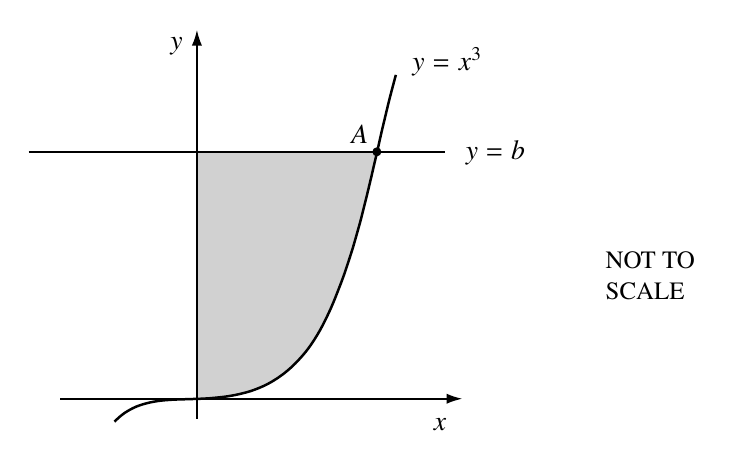
\begin{tikzpicture}[x=0.0127cm,y=-0.0127cm,font=\normalsize]
  % shaded region: y-axis, line y = b, curve
  \fill[shade] (254.5,166) -- (254.5,413) -- plot[smooth] coordinates {(255,413) (260.6,413.1) (266.1,412.9) (271.6,412.6) (277.1,412.1) (282.5,411.5) (287.9,410.6) (293.2,409.6) (298.5,408.3) (303.6,406.9) (308.7,405.2) (313.7,403.4) (318.6,401.3) (323.4,399) (328.1,396.5) (332.6,393.9) (337.1,391) (341.3,387.9) (345.4,384.7) (349.3,381.2) (353.1,377.6) (356.8,373.8) (360.3,369.7) (363.7,365.5) (367,361.1) (370.1,356.6) (373.2,351.9) (376,347.1) (378.8,342.2) (381.5,337.2) (384.1,332.1) (386.6,326.9) (389,321.6) (391.3,316.3) (393.6,310.8) (395.7,305.4) (397.8,299.9) (399.8,294.3) (401.8,288.7) (403.7,283.1) (405.5,277.4) (407.3,271.7) (409.1,266) (410.8,260.2) (412.5,254.4) (414.1,248.5) (415.8,242.6) (417.4,236.7) (419,230.9) (420.5,225) (422.1,219.1) (423.6,213.3) (425.1,207.4) (426.5,201.4) (428,195.5) (429.3,189.6) (430.7,183.8) (432,177.9) (433.3,172) (434.5,166)} -- cycle;
  \draw[->] (118,413) -- (520,413);
  \draw[->] (254.5,433) -- (254.5,44);
  \draw (86,166) -- (503,166);
  \draw[line width=0.9pt] plot[smooth] coordinates {(172,436) (176.9,431.3) (182.2,427.2) (187.8,423.8) (193.8,420.9) (200.3,418.6) (207.2,416.8) (214.7,415.4) (222.7,414.5) (231.2,413.9) (240.1,413.6) (249.6,413.3) (258.7,413) (267.4,412.5) (276,411.7) (284.4,410.7) (292.6,409.3) (300.5,407.5) (308.1,405.4) (315.2,402.8) (322.2,399.8) (328.8,396.3) (335.2,392.3) (341.5,387.8) (347.5,382.8) (353.2,377.4) (358.6,371.6) (363.7,365.6) (368.5,359.1) (372.9,352.4) (377.2,345.2) (381.2,337.7) (385,330) (388.7,322) (392.2,313.7) (395.5,305.3) (398.8,296.8) (401.9,288.3) (404.8,279.7) (407.6,271.1) (410.4,262.3) (413,253.3) (415.5,244.5) (418,235.5) (420.3,226.5) (422.6,217.4) (424.8,208.4) (427,199.2) (429.2,190) (431.3,180.8) (433.5,171.4) (435.6,162.2) (437.7,152.8) (439.8,143.6) (442,134.4) (444.2,125.2) (446.4,116.1) (448.7,107.1) (451.1,98.01) (453.5,89)};
  \fill (434.5,166) circle (4.5);
  \node at (417,149) {$A$};
  \node at (553,167) {$y=b$};
  \node at (505,76) {$y=x^3$};
  \node at (497,439) {$x$};
  \node at (234,60) {$y$};
  \node[align=left,font=\small] at (708,290) {NOT TO\\SCALE};
\end{tikzpicture}
\end{document}
